\subsection{Scenario 3}

\begin{frame}{Results}{Scenario 3 - Above the GS}

  \begin{block}{Goal}
	Describing the movement of the antennas when the UA is flying above the GS.
  \end{block}

  \begin{figure}[H]
    \centerline{
    \subfigure[UAS Map]{
    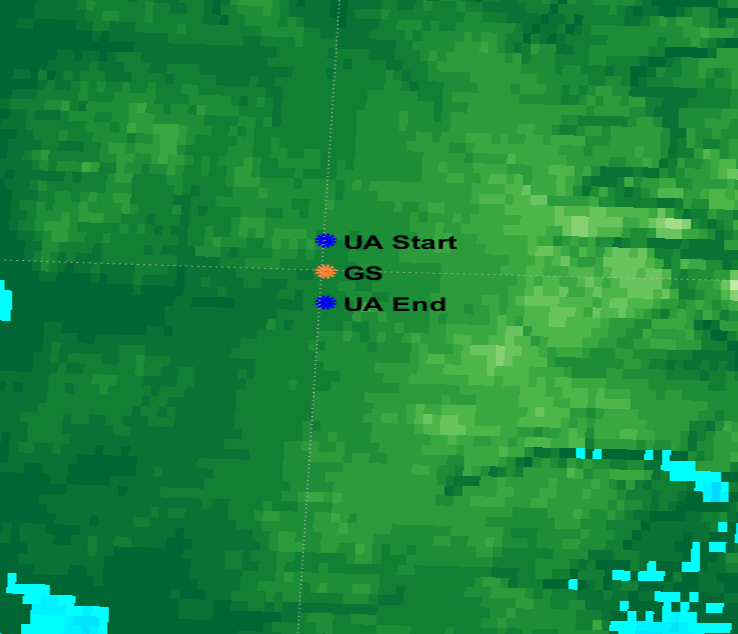
\includegraphics[scale=0.25]{figures/s3_zoom.png}}
    \hfill
    \subfigure[Distance between UA and GS]{
    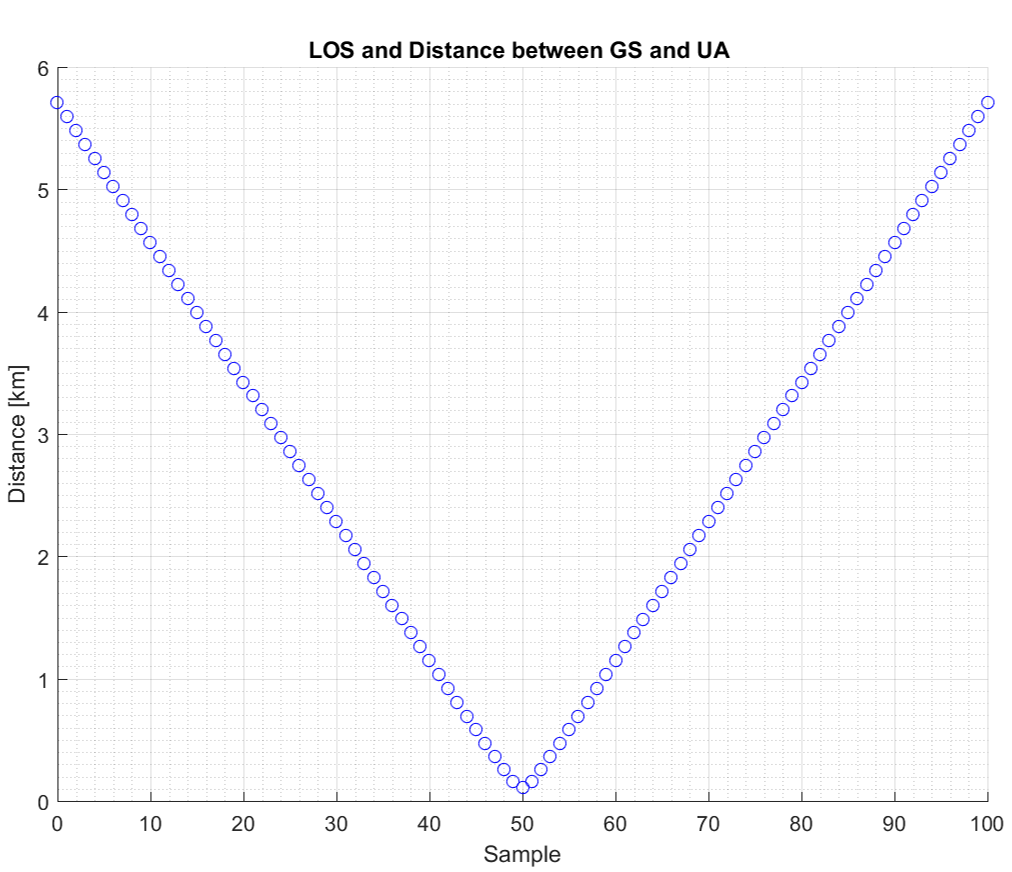
\includegraphics[scale=0.35]{figures/s3_los.png}}}
  \end{figure}

\end{frame}



\begin{frame}{Results}{Scenario 3 - Above the GS}

  \begin{block}{GS Tracking Angles}  
  
  \begin{figure}[H]
    \centerline{
    \subfigure[UAS Map]{
    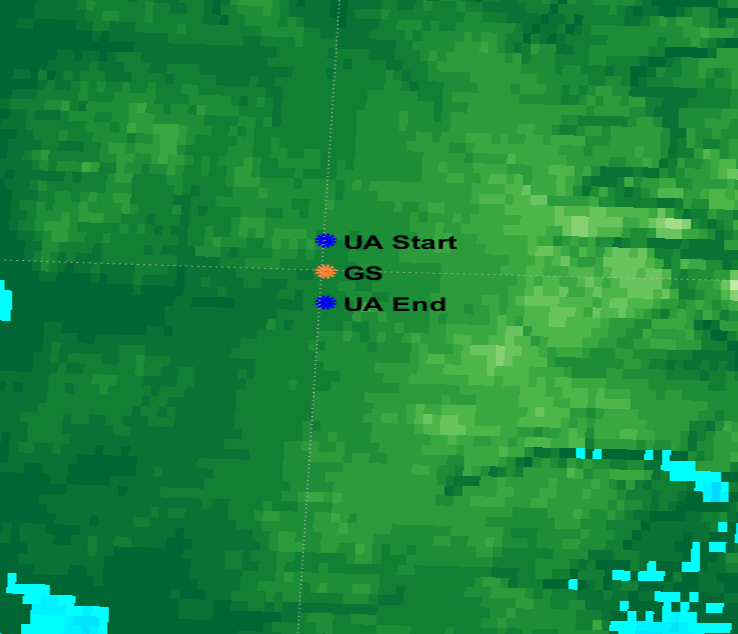
\includegraphics[scale=0.25]{figures/s3_zoom.png}}
    \hfill
    \subfigure[Azimuth and elevation angles of the antenna on the GS]{
    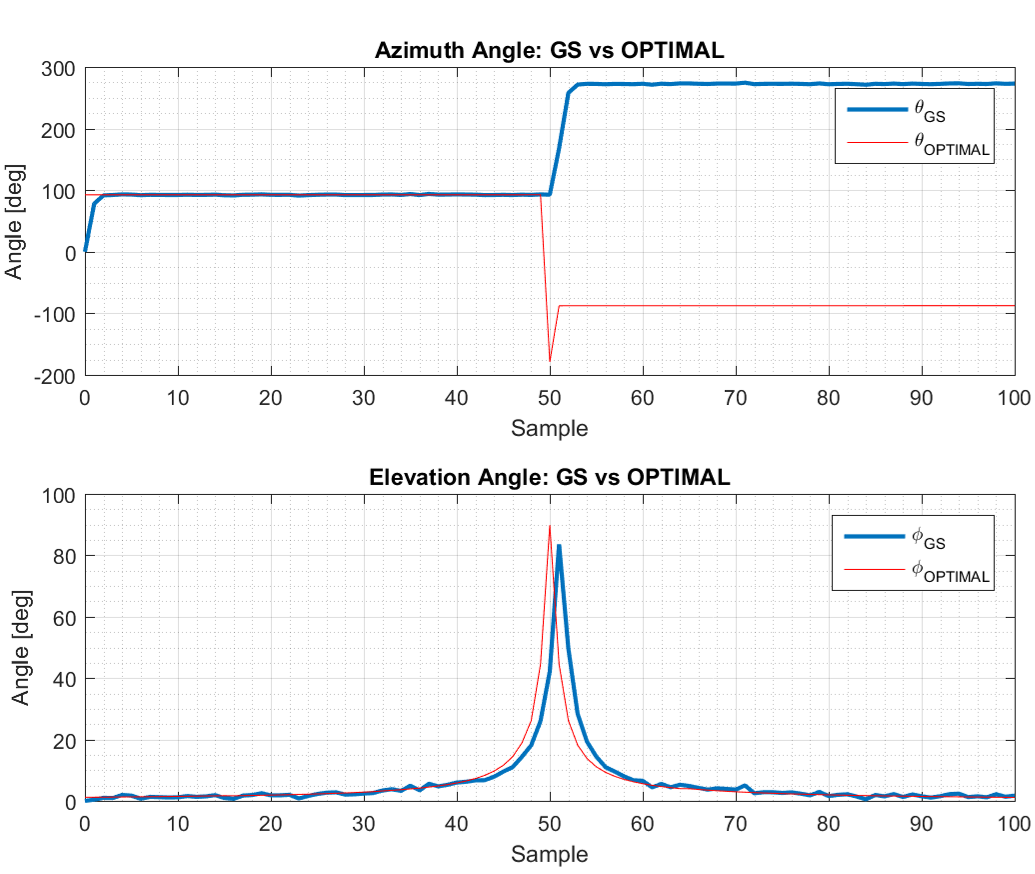
\includegraphics[scale=0.35]{figures/s3_gs.png}}}
  \end{figure}
  
  \end{block}

\end{frame}



\begin{frame}{Results}{Scenario 3 - Above the GS}

  \begin{block}{UA Tracking Angles}  
  
  \begin{figure}[H]
    \centerline{
    \subfigure[UAS Map]{
    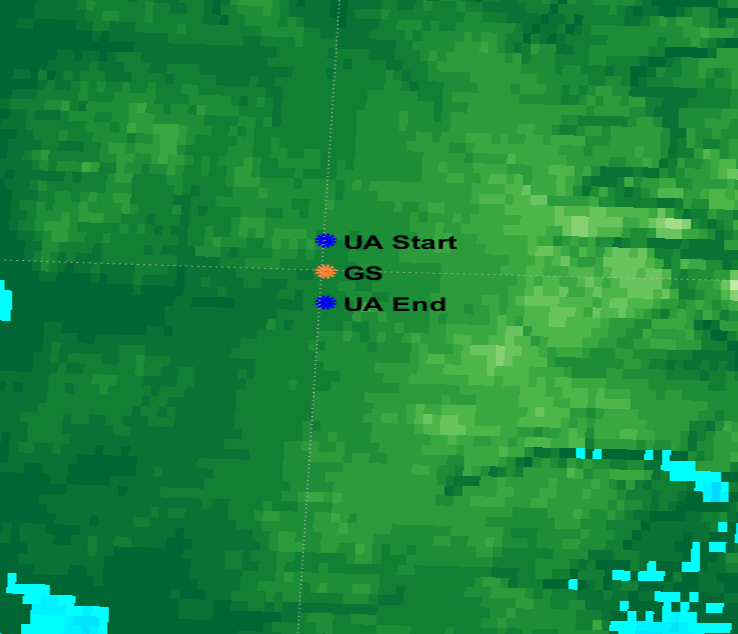
\includegraphics[scale=0.25]{figures/s3_zoom.png}}
    \hfill
    \subfigure[Azimuth and elevation angles of the antenna on the UA]{
    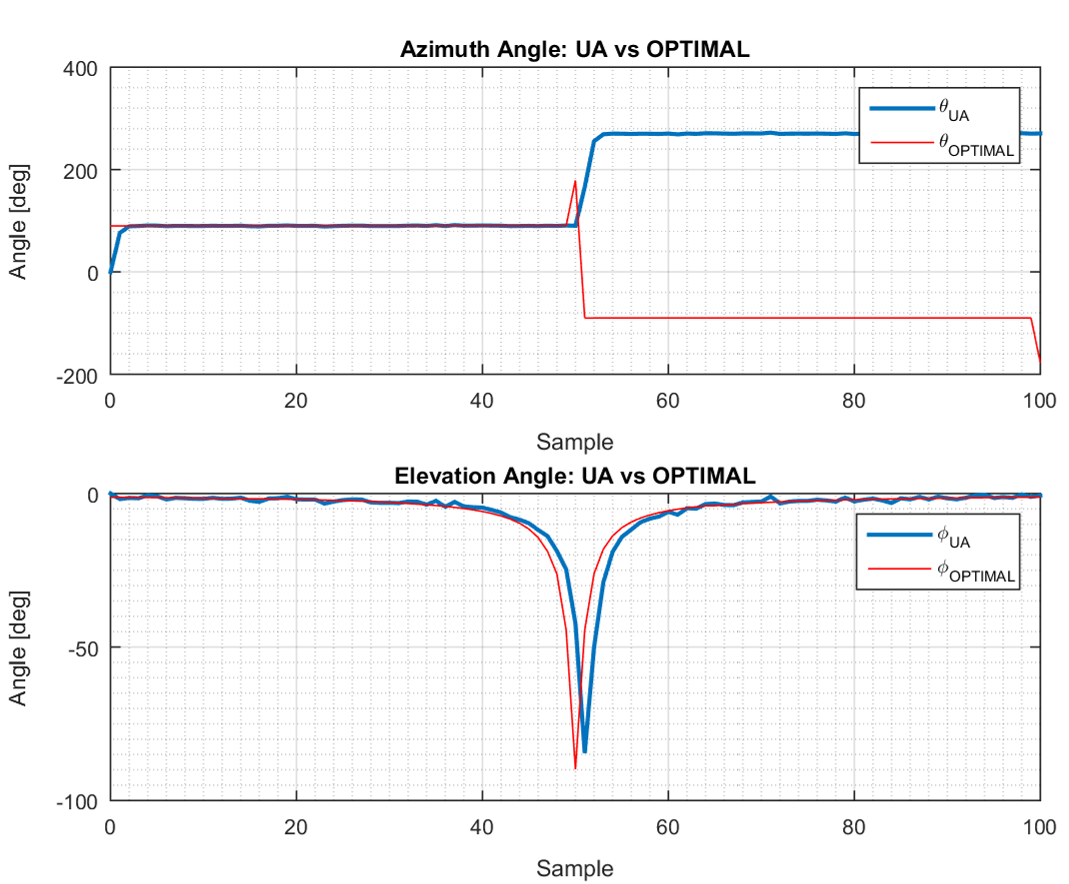
\includegraphics[scale=0.35]{figures/s3_ua.png}}}
  \end{figure}
  
  \end{block}

\end{frame}



\begin{frame}{Results}{Scenario 3 - Above the GS}

  \begin{block}{Signal Power}  
  
  \begin{figure}[H]
    \centerline{
    \subfigure[UAS Map]{
    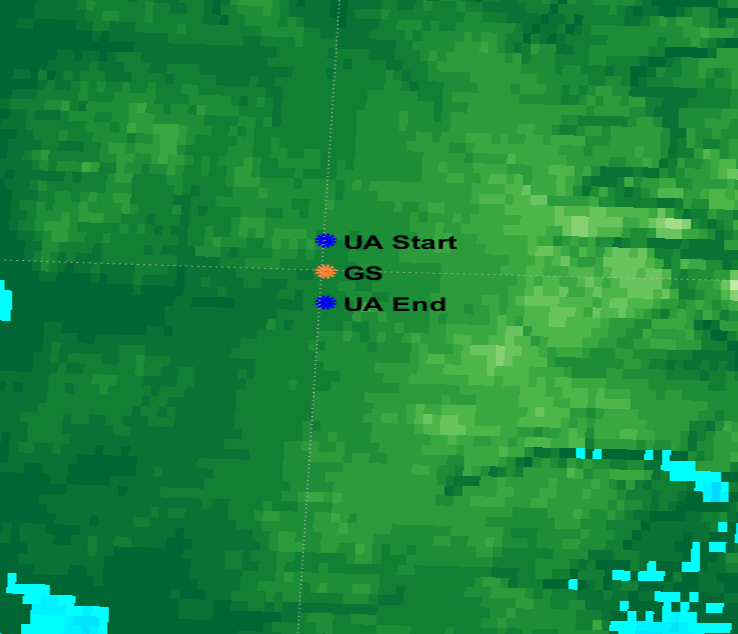
\includegraphics[scale=0.25]{figures/s3_zoom.png}}
    \hfill
    \subfigure[Power at the receiver]{
    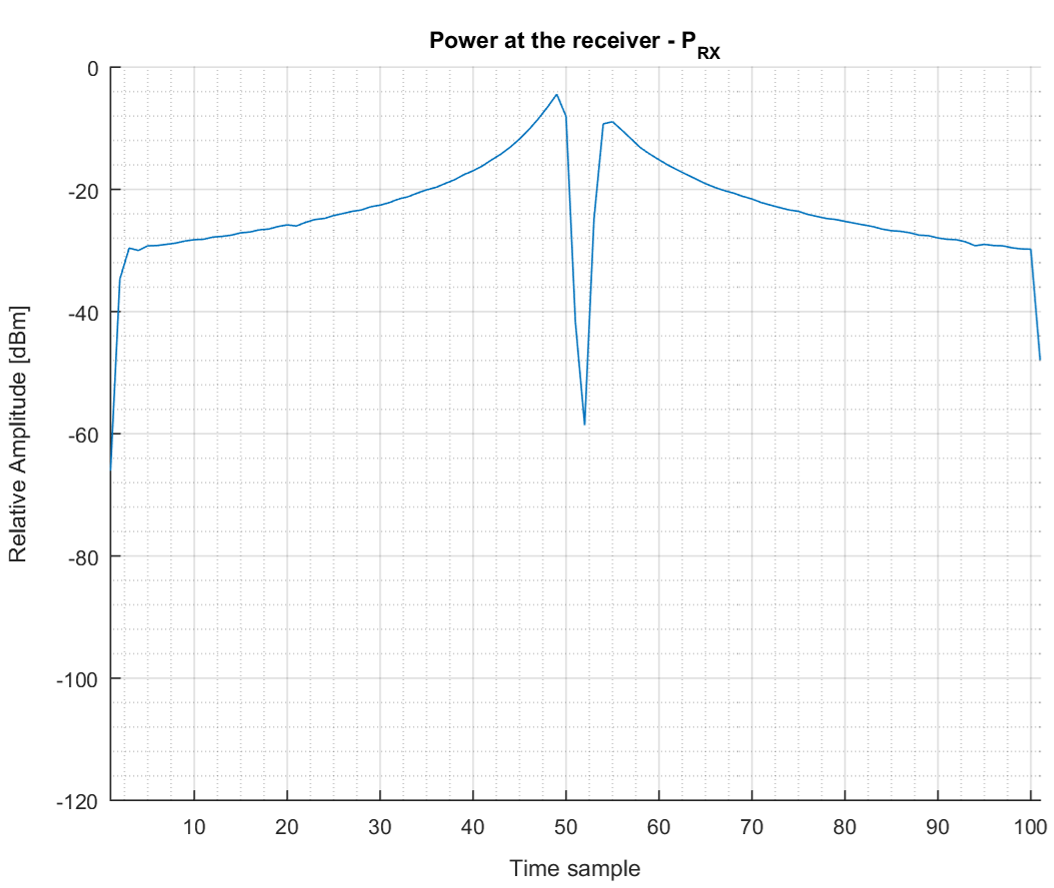
\includegraphics[scale=0.35]{figures/s3_power.png}}}
  \end{figure}
  
  \end{block}

\end{frame}
